% !TeX spellcheck = en_US
\documentclass[11pt,a4paper]{scrartcl}
%\documentclass[11pt,a4paper]{article}
\usepackage{longtable}
\usepackage{verbatim}
\usepackage{amsmath}
\usepackage{amssymb}
\usepackage{amstext}
\usepackage{graphicx}
\usepackage{graphics} %for resizebox
\usepackage{xcolor}
\usepackage{caption}
\usepackage[update]{epstopdf}
\usepackage{subfig} % Layout wird weiter unten festgelegt !
\usepackage{natbib}
\usepackage{dcolumn}
\usepackage{booktabs}
\usepackage{tabularx}
\usepackage{multicol}
%\usepackage{a4wide}
\usepackage{threeparttable}
\usepackage[countmax]{subfloat}
%\usepackage[capposition=top]{floatrow} %for notes an figures
\usepackage{float}             % Stellt die Option [H] fuer Floats zur Verfgung
\usepackage{eurosym} %um Eurozeichen darzusellen
%%% Doc: No Documentation
\usepackage{flafter}          % Floats immer erst nach der Referenz setzen
\usepackage{textcomp}
\usepackage[update]{epstopdf}
\usepackage[update]{psfrag}
\usepackage{wrapfig}
\usepackage{mdframed}
% Defines a \FloatBarrier command, beyond which floats may not
% pass; useful, for example, to ensure all floats for a section
% appear before the next \section command.

\usepackage[
	section		% "\section" command will be redefined with "\FloatBarrier"
]{placeins}

\usepackage{afterpage}

\usepackage{geometry}
\geometry{a4paper,left=30mm, right=30mm, top=30mm, bottom=30mm}


\usepackage[latin1]{inputenc}
% \usepackage[T1]{fontenc} % Makes T small. disabled.
\usepackage{pdflscape}
%%% Doc: ftp://tug.ctan.org/pub/tex-archive/macros/latex/contrib/hyperref/doc/manual.pdf
\usepackage[
%   % Farben fuer die Links
   breaklinks,
   colorlinks,         % Links erhalten Farben statt Kaeten
   urlcolor=purple,
   citecolor=blue,
   linkcolor=violet,
   bookmarks=true,          % Erzeugung von Bookmarks fuer PDF-Viewer
   % PDF Informationen
   pdftitle={Add a pdf title},             % Titel
   pdfauthor={Philipp Grosskurth}            % Autor
   pdfcreator={LaTeX, hyperref, KOMA-Script}, % Ersteller
   pdfkeywords={PG},
%   %pdfproducer={pdfeTeX 1.10b-2.1} %Produzent
   pdfdisplaydoctitle=true, % Dokumententitel statt Dateiname im Fenstertitel
   pdfstartview=FitH,       % Dokument wird Fit Width geaefnet
   pdfpagemode=UseOutlines, % Bookmarks im Viewer anzeigen
   pdfpagelabels=true,           % set PDF page labels
%   pdfpagelayout=TwoPageRight, % zweiseitige Darstellung: ungerade Seiten
%   									 % rechts im PDF-Viewer
%   %pdfpagelayout=SinglePage, % einseitige Darstellung
]{hyperref}

%% Zeilenabstand =========================================================
%
%%% Doc: ftp://tug.ctan.org/pub/tex-archive/macros/latex/contrib/setspace/setspace.sty
\usepackage{setspace}
\onehalfspacing		% 1,5-facher Abstand
%\doublespacing		% 2-facher Abstand
% hereafter load 'typearea' again



\bibliographystyle{joephd3}
%\DeclareGraphicsRule{.eps}{eps}{*}{}

%\newtheorem{thm}{Theorem}
%\newtheorem{prop}{Proposition}
%\newtheorem{lem}{Lemma}
%\newtheorem{ass}{Assumption}
%\newtheorem{cor}{Corollary}
%\newtheorem{ex}{Example}
%\newtheorem{defn}{Definition}
%\newtheorem{case}{Case}

%\newenvironment{proof}{\noindent \textbf{Proof}. }{ \hspace*{\fill} $\blacksquare$ \newline}

%\newcommand{\superscript}[1]{\ensuremath{^{\textrm{#1}}}}
%\newcommand{\th}[0]{\superscript{th}}
%\newcommand{\st}[0]{\superscript{st}}
%\newcommand{\nd}[0]{\superscript{nd}}
%\newcommand{\rd}[0]{\superscript{rd}}
\def\sym#1{\ifmmode^{#1}\else\(^{#1}\)\fi}
\newcommand\MC[1]{\multicolumn{1}{c}{#1}}
\newcolumntype{d}[1]{D{.}{.}{#1}}
\newcolumntype{C}{>{\centering\arraybackslash}X}
\newcolumntype{L}{>{\centering}p{4.5cm}}

% Allow line breaks with \\ in specialcells
\newcommand{\specialcell}[2][l]{\begin{tabular}[#1]{@{}l@{}}#2\end{tabular}}


%\renewcommand{\baselinestretch}{1.2}

\begin{document}
\singlespacing

\title{Add a title here.\thanks{Add acknowledgements here.}}

%\date{-- Preliminary version -- \\ -- Please do not cite or distribute -- }
\date{Add a date here}

\author{Philipp Gro{\ss}kurth\thanks{RWI, philipp.grosskurth@rwi-essen.de}}

\maketitle\thispagestyle{empty}

%ist schonmal drauf, aber eher etwas klein ;)
%\begin{figure}
%\centering
%\includegraphics[width=0.25\textwidth]{logo_eib.eps}
%\label{fig:logo_eib}
%\end{figure}


%\newpage
\begin{abstract}

\noindent\textbf{Abstract}: Add an abstract here.
\\

\noindent\textbf{Keywords}: Some keywords \\
\noindent\textbf{JEL Classification}: STFU  \\

\end{abstract}

%\end{flushleft}
\doublespacing		% 2-facher Abstand
%\doubles
\newpage
\pagestyle{plain}
\pagenumbering{arabic}

\tableofcontents
\newpage
%$$$$$$$$$$$$$$$$$$$$$$$$$$$$$$$$$$$$$$$$$$$$$$$$$$$$
\section{Introduction}\label{sec:introduction}
%$$$$$$$$$$$$$$$$$$$$$$$$$$$$$$$$$$$$$$$$$$$$$$$$$$$$


The Witness is a 3D puzzle video game developed and published by Thekla, Inc.[a] It was released for Microsoft Windows and PlayStation 4 in January 2016, and later for Xbox One, Nvidia Shield, macOS, and iOS. Inspired by Myst, the game involves the exploration of an open world island filled with natural and man-made structures. The player progresses by solving puzzles, which are based on interactions with mazes presented on panels around the island or hidden within the environment. The player will have to determine the rules of each puzzle from visual clues and audio recordings scattered around the island.

Jonathan Blow, the game's lead designer, desired to create a game around non-verbal communication, wanting players to learn from observation and to come to epiphanies in finding solutions and leading to a greater sense of involvement and accomplishment with each success. The game includes around 650 puzzles, though the player is not required to solve them all to finish the game.

Originally announced in 2009, The Witness had a lengthy development period. Blow started work on the title in 2008 shortly after releasing Braid. The financial success of Braid allowed him to hire a larger production team without ceding control over the final product. In order to create the game's visual language, the team developed their own game engine and retained artists, architects, and landscape architects to design the structures on the island. This required a protracted development process, and the game's release was delayed from 2013 to 2016. Original plans for release on the PlayStation 3 and Xbox 360 were abandoned as the game engine became more demanding, and the team ultimately opted for an initial release on Windows and the PlayStation 4, with support for other platforms following.

The Witness received widespread acclaim from critics, who praised the difficult but surmountable puzzles and the game's art and setting. Within a week of release, the game had sold over 100,000 copies, which was about as many copies as Braid had done within a year of its release, nearly recouping all of the development costs for the game.

Here's a source: \citet{Kalemli-Ozcan2015} \\

%$$$$$$$$$$$$$$$$$$$$$$$$$$$$$$$$$$$$$$$$$$$$$$$$$$$$
\section{Data and Methodology}\label{sec:datamethod}
%$$$$$$$$$$$$$$$$$$$$$$$$$$$$$$$$$$$$$$$$$$$$$$$$$$$$

The Witness is a 3D puzzle video game developed and published by Thekla, Inc.[a] It was released for Microsoft Windows and PlayStation 4 in January 2016, and later for Xbox One, Nvidia Shield, macOS, and iOS. Inspired by Myst, the game involves the exploration of an open world island filled with natural and man-made structures. The player progresses by solving puzzles, which are based on interactions with mazes presented on panels around the island or hidden within the environment. The player will have to determine the rules of each puzzle from visual clues and audio recordings scattered around the island.

\begin{figure}[htp]
	\centering
		\psfrag{0}[c][c][1][0]{\normalsize 0}
\psfrag{.2}[c][c][1][0]{\normalsize .2}
\psfrag{.4}[c][c][1][0]{\normalsize .4}
\psfrag{.6}[c][c][1][0]{\normalsize .6}
\psfrag{.8}[c][c][1][0]{\normalsize .8}
\psfrag{1}[c][c][1][0]{\normalsize 1}
\psfrag{Share of constant information}[c][c][1][0]{\normalsize Share of constant information}
\psfrag{2002}[c][c][1][0]{\normalsize 2002}
\psfrag{2004}[c][c][1][0]{\normalsize 2004}
\psfrag{2006}[c][c][1][0]{\normalsize 2006}
\psfrag{2008}[c][c][1][0]{\normalsize 2008}
\psfrag{2010}[c][c][1][0]{\normalsize 2010}
\psfrag{2012}[c][c][1][0]{\normalsize 2012}
\psfrag{Year}[c][c][1][0]{\normalsize Year}
\psfrag{Ownership information stability, 2012-2002}[c][c][1][0]{\normalsize Ownership information stability, 2012-2002}
\psfrag{Original}[l][l][1][0]{\normalsize Original}
\psfrag{With carryforward}[l][l][1][0]{\normalsize With carryforward}
 % change path to output/ and adjust filename accordingly
		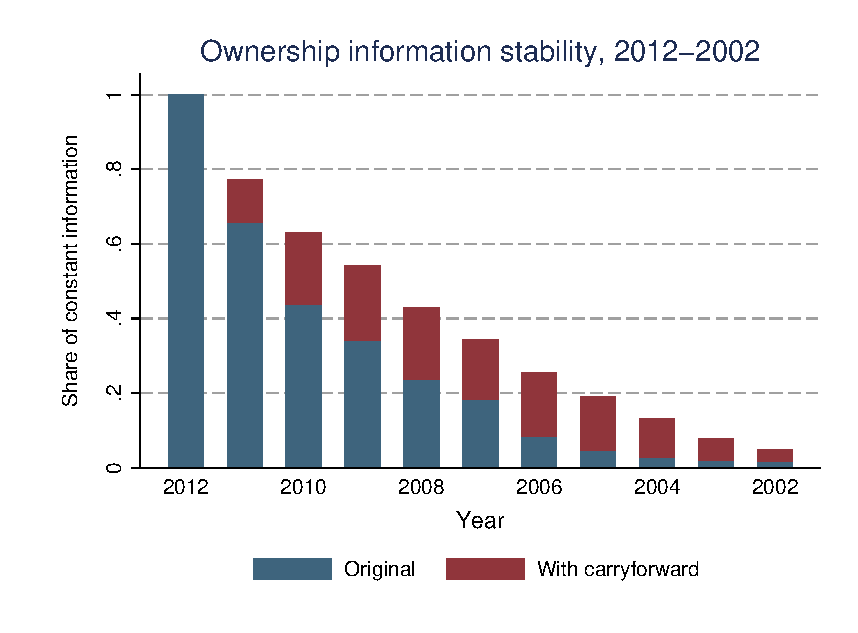
\includegraphics[width=\textwidth]{input/testfigure.eps} % change path to output/ and adjust filename accordingly
	\caption{A testfigure}
	\label{fig:testfigure} % make sure the name of the figure never changes
\end{figure}

Jonathan Blow, the game's lead designer, desired to create a game around non-verbal communication, wanting players to learn from observation and to come to epiphanies in finding solutions and leading to a greater sense of involvement and accomplishment with each success. The game includes around 650 puzzles, though the player is not required to solve them all to finish the game.

Originally announced in 2009, The Witness had a lengthy development period. Blow started work on the title in 2008 shortly after releasing Braid. The financial success of Braid allowed him to hire a larger production team without ceding control over the final product. In order to create the game's visual language, the team developed their own game engine and retained artists, architects, and landscape architects to design the structures on the island. This required a protracted development process, and the game's release was delayed from 2013 to 2016. Original plans for release on the PlayStation 3 and Xbox 360 were abandoned as the game engine became more demanding, and the team ultimately opted for an initial release on Windows and the PlayStation 4, with support for other platforms following.

The Witness received widespread acclaim from critics, who praised the difficult but surmountable puzzles and the game's art and setting. Within a week of release, the game had sold over 100,000 copies, which was about as many copies as Braid had done within a year of its release, nearly recouping all of the development costs for the game.

%$$$$$$$$$$$$$$$$$$$$$$$$$$$$$$$$$$$$$$$$$$$$$$$$$$$$
\section{Results}\label{sec:results}
%$$$$$$$$$$$$$$$$$$$$$$$$$$$$$$$$$$$$$$$$$$$$$$$$$$$$

The Witness is a 3D puzzle video game developed and published by Thekla, Inc.[a] It was released for Microsoft Windows and PlayStation 4 in January 2016, and later for Xbox One, Nvidia Shield, macOS, and iOS. Inspired by Myst, the game involves the exploration of an open world island filled with natural and man-made structures. The player progresses by solving puzzles, which are based on interactions with mazes presented on panels around the island or hidden within the environment. The player will have to determine the rules of each puzzle from visual clues and audio recordings scattered around the island.

\begin{center}
	\resizebox{\linewidth}{!}{ % resize the table to match the line width - adjust if necessary
		\begin{tabular}{lrrrrrrrrrrrr}
\hline
 & \multicolumn{12}{c}{\textbf{Year, 2005-2012}} \\
\textbf{GUO similarity} & \multicolumn{3}{c}{\textbf{2005}} & \multicolumn{3}{c}{\textbf{2006}} & \multicolumn{3}{c}{\textbf{2007}} & \multicolumn{3}{c}{\textbf{Total}} \\
&No.&\%&\%&No.&\%&\%&No.&\%&\%&No.&\%&\% \\
\hline
matched hit&2,388&32.8&32.8&2,433&33.4&33.4&2,814&38.7&38.7&7,635&35.0&35.0 \\
matched miss&3,601&49.5&82.3&3,716&51.1&84.5&3,066&42.1&80.8&10,383&47.5&82.5 \\
mismatched miss&333&4.6&86.9&158&2.2&86.6&356&4.9&85.7&847&3.9&86.4 \\
mismatched hit&603&8.3&95.1&662&9.1&95.7&588&8.1&93.7&1,853&8.5&94.9 \\
other GUO found&354&4.9&100.0&310&4.3&100.0&455&6.3&100.0&1,119&5.1&100.0 \\
\textbf{Total}&7,279&100.0&&7,279&100.0&&7,279&100.0&&21,837&100.0& \\
\hline
\end{tabular}
 % change path to output/ and adjust filename accordingly
	}
\end{center}


Jonathan Blow, the game's lead designer, desired to create a game around non-verbal communication, wanting players to learn from observation and to come to epiphanies in finding solutions and leading to a greater sense of involvement and accomplishment with each success. The game includes around 650 puzzles, though the player is not required to solve them all to finish the game.

Originally announced in 2009, The Witness had a lengthy development period. Blow started work on the title in 2008 shortly after releasing Braid. The financial success of Braid allowed him to hire a larger production team without ceding control over the final product. In order to create the game's visual language, the team developed their own game engine and retained artists, architects, and landscape architects to design the structures on the island. This required a protracted development process, and the game's release was delayed from 2013 to 2016. Original plans for release on the PlayStation 3 and Xbox 360 were abandoned as the game engine became more demanding, and the team ultimately opted for an initial release on Windows and the PlayStation 4, with support for other platforms following.

The Witness received widespread acclaim from critics, who praised the difficult but surmountable puzzles and the game's art and setting. Within a week of release, the game had sold over 100,000 copies, which was about as many copies as Braid had done within a year of its release, nearly recouping all of the development costs for the game.

%$$$$$$$$$$$$$$$$$$$$$$$$$$$$$$$$$$$$$$$$$$$$$$$$$$$$
\section{Conclusion}\label{sec:conclusion}
%$$$$$$$$$$$$$$$$$$$$$$$$$$$$$$$$$$$$$$$$$$$$$$$$$$$$

The Witness is a 3D puzzle video game developed and published by Thekla, Inc.[a] It was released for Microsoft Windows and PlayStation 4 in January 2016, and later for Xbox One, Nvidia Shield, macOS, and iOS. Inspired by Myst, the game involves the exploration of an open world island filled with natural and man-made structures. The player progresses by solving puzzles, which are based on interactions with mazes presented on panels around the island or hidden within the environment. The player will have to determine the rules of each puzzle from visual clues and audio recordings scattered around the island.

\newpage
%\phantomsection
\addcontentsline{toc}{section}{References}
\bibliography{library/library}



\newpage
\appendix

%$$$$$$$$$$$$$$$$$$$$$$$$$$$$$$$$$$$$$$$$$$$$$$$$$$$$
\section{Appendix}\label{sec:appendix}
%$$$$$$$$$$$$$$$$$$$$$$$$$$$$$$$$$$$$$$$$$$$$$$$$$$$$

The Witness is a 3D puzzle video game developed and published by Thekla, Inc.[a] It was released for Microsoft Windows and PlayStation 4 in January 2016, and later for Xbox One, Nvidia Shield, macOS, and iOS. Inspired by Myst, the game involves the exploration of an open world island filled with natural and man-made structures. The player progresses by solving puzzles, which are based on interactions with mazes presented on panels around the island or hidden within the environment. The player will have to determine the rules of each puzzle from visual clues and audio recordings scattered around the island.

\end{document}



%%%%%%%%%%%%%%%%%%%%%%%%%%%%%%%%%%%%%%%%%%%%%%%%%%%%%%%%%%
